\documentclass{acm_proc_article-sp}
\usepackage{color}
\usepackage{comment}

\newcommand{\bu}[1]{{\color{red}#1}}

\begin{document}

\title{Exploiting Resource Diversity in the Public Cloud to Offer Performance Modeling as a Service (PMaaS)}

\numberofauthors{1}
\author{
% You can go ahead and credit any number of authors here,
% e.g. one 'row of three' or two rows (consisting of one row of three
% and a second row of one, two or three).
%
% The command \alignauthor (no curly braces needed) should
% precede each author name, affiliation/snail-mail address and
% e-mail address. Additionally, tag each line of
% affiliation/address with \affaddr, and tag the
% e-mail address with \email.
%
% 1st. author
\alignauthor
Mark Meredith\\
       \affaddr{Penn State Computer Science and Engineering Department}\\
       \affaddr{769 Tanager Dr}\\
       \affaddr{State College, PA 16803}\\
       \email{mwm126@gmail.com}
}
% There's nothing stopping you putting the seventh, eighth, etc.
% author on the opening page (as the 'third row') but we ask,
% for aesthetic reasons that you place these 'additional authors'
% in the \additional authors block, viz.
\additionalauthors{Additional authors: John Smith (The Th{\o}rv{\"a}ld Group,
email: {\texttt{jsmith@affiliation.org}}) and Julius P.~Kumquat
(The Kumquat Consortium, email: {\texttt{jpkumquat@consortium.net}}).}
\date{30 July 1999}
% Just remember to make sure that the TOTAL number of authors
% is the number that will appear on the first page PLUS the
% number that will appear in the \additionalauthors section.

\maketitle
\begin{abstract}
One of the main benefits of virtualization through cloud computing is the ready availability of large rapid virtual machines for rapid application deployment. As computing hardware advances, cloud computing vendors offer new virtual machines with new performance characteristics, adding to the large set of virtual machine types to choose from. Many virtual machine types are available, with varying performance and pricing options. In this work we present a statistical model for estimating the performance of new virtual machine types based on knowledge of existing types. This model is based on data collected by running the Yahoo! Cloud Services Benchmark (YCSB). The databases surveyed are the key-value database Redis, deployed on Amazon Elasticache, and the NoSQL databases Apache Cassandra, deployed on Amazon Elastic Compute Cloud. We tested these on a variety of Amazon virtual machines types.

\end{abstract}

\keywords{Performance modeling, public cloud, regression, empirical evaluation} % NOT required for Proceedings

\section{Introduction}

%Cloud vendors offer a lot of different virtual machine instance types. Cloud tenants needs to determine what benefit new virtual machine types will bring to their applications.

~\bu{Many enterprises are choosing to migrate their information technology (IT) needs to public cloud computing platforms, a trend that is projected to continue anabated in the foreseeable future~\cite{xxx}. 

}


Solution: test your application on different VM types and find out?

present the problem, its significance, and key challenges
 
explain why the state-of-the-art may not be adequate, particularly as clouds move towards higher levels of utilization and dynamism

explain our key ideas and contributions

\section{Background}
big picture overview of tenant-side decision-making, where PMaaS fits within this, mention the specific assumptions we make, the chosen environment, which ideas are likely to generalize to other settings
 
what about the costs of PMaaS itself? how to make it practical? might providers actually offer it as a service?

\subsection{Methodology}

We benchmarked virtual machines on the oldest and most widely used cloud vendor, Amazon Web Services (AWS).

We studied three different types of databases: Apache Cassandra (NoSQL database), Redis (Key-Value caching database), and MySQL (SQL database).

We used the Yahoo! Cloud Serving Benchmark (YCSB) to profile the behavior of these three databases.

We ran the YCSB client on a m4.2xlarge EC2 instance running Ubuntu Linux 14.04. We monitored the system load average on the client machine to verify that the client was not the bottleneck during the tests.

\begin{itemize}
\item multiple linear regression on data for 3 VM types
\item use model to get predicted residuals for 1 VM type
\item add data for other VM types to the model
\item note that the residual decreases when fitting model to more terms
\end{itemize}

\begin{table}
\centering
\caption{AWS instance types}
\begin{tabular}{|r|l|c|r|l|} \hline
Abbreviation&Name& \# cores&Memory&Network\\ \hline
$VM_1$ & r3.large & 2 & 15 GB & Moderate\\ \hline
$VM_2$ & r3.xlarge & 4 & 30.5 GB & Moderate\\ \hline
$VM_3$ & r3.2xlarge & 8 & 61 GB & High\\ \hline
$VM_4$ & m3.large & 2 & 7.5 GB & Moderate\\ \hline
$VM_5$ & m3.xlarge & 4 & 15 GB & Moderate\\ \hline
$VM_6$ & m3.2xlarge & 8 & 30 GB & High\\ \hline
\hline\end{tabular}
\label{table:rdstypes}
\end{table}

\subsection{Predictive Residual}

For multiple linear regressions, the coefficient of determination $R^2$ always increases when adding independent variables.  A better measure of goodness of fit is for our model is predicted $R^2$, defined in terms of PRESS statistic, which in turn is defined in terms of 

We model the latency vs. throughput at low levels of throughput, where the relationship is linear (see Figure TODO).

We do a multiple linear regression on the parameters in Table XXX for the data from a set of VM instance types to get a linear regression model $y_i = \beta_1 x_i1+\dotfill+\beta_{p}x_{ip}$

We use the model to find predicted values for the test instance type.

As more VM instances are added to training data, the model fits better for predicting values for the test instance type.  The goodness of fit is defined as the normalized residual:

\newdef{definition}{Definition}
\begin{definition}
Predicted Residual
\begin{displaymath}{
Predicted Residual=\sum_{i=1}^{n} (y_i - \hat{y}(x_i))^{2}
}\end{displaymath}

\end{definition}

The residual is normalized with the total sum of squares for the test data from the mean.

\begin{definition}
TSS (Total Sum of Squares)
\begin{displaymath}{
TSS=\sum_{i=1}^{n} (y_i - \bar{y})^{2}
}\end{displaymath}

\begin{displaymath}{
R_{predicted}^2 = (1 - PredictedResidual/TSS)
}\end{displaymath}
\end{definition}

 \section{Case Studies}

\subsection{Apache Cassandra}

Apache Cassandra is a Table/Key-Value hybrid NoSQL database.

Apache Cassandra was installed on Amazon EC2 instances of various VM instance types. The Cassandra cluster varied in size from 1 node to 5 nodes.

\begin{itemize}
   \item present linear regression model, explain simplifications, justifications
   \item present non-linear regression model if applicable
\end{itemize}

\subsubsection{Evaluation for a Strict Consistency Configuration}

\begin{itemize}
\item replication factor=1 (crashes for >1)
\item consistency N/A (ONE==ALL)
\end{itemize}
Workload B (95/5 r/w) with uniform distribution

Present data for
7 gen VM types, 3 workloads, 1-5 nodes, replication factor 1

\subsubsection{Evaluation for a Weak Consistency Configuration}

consistency=ONE

Workload B (95/5 r/w) with uniform distribution

Present data for
3 VM types: gen,mem,cpu, throughputs 5000-20000, replication factor 3, 5 nodes

\subsection{Redis}

Redis is a key-value NoSQL database.

Redis was deployed on AWS using Amazon ElastiCache, a web service that abstracts the deployment and administration of the OS and database software.

Redis was tested using YCSB Workload B (95\% read/5\% write) with zipfian distribution.

We observed the latency at various throughputs and VM instance types.

Latency increases slowly at low throughputs, and then rapidly increases near the load capacity of the database.

fit nonlinear model to find transition point at each configuration
The throughput at which it transitions should increase with faster VMs or higher node counts  
fit linear model to (transition throughput, nodes) for a select VM type

We used VM type r3.2xlarge as test data, while increasing the training data in Table \ref{table:redis} and Figure \ref{figure:redisbarread}.  The fit improves as more VMs are added to the training set, as shown in Figure \ref{figure:redisread} and Figure \ref{figure:rediswrite}.

\begin{table}
\centering
\caption{Redis $R_{predicted}^2$ for $VM_6$}
\begin{tabular}{|r|r|l|} \hline
$R_{read}^2$&$R_{write}^2$&Training Data\\ \hline
-0.657113 & -0.573816 & $VM_1$\\ \hline
0.155888 & 0.0674494 & $VM_1,VM_2$\\ \hline
0.43653 & 0.395256 & $VM_1,VM_2,VM_3$\\ \hline
0.783798 & 0.727331 & $VM_1,VM_2,VM_3,VM_4$\\ \hline
0.80571 & 0.748588 & $VM_1,VM_2,VM_3,VM_4,VM_5$\\ \hline
%0.86354 & 0.836441 & $VM_1,VM_2,VM_3,V_4,V_5,V_6$\\ \hline
\hline\end{tabular}
\label{table:redis}
\end{table}

\newcommand{barfigure}[2] {
\begin{figure}
\centering
\includegraphics[scale = 0.5]{#1}
\caption{#2}
\label{figure:redisbarread}
\end{figure}
}

\newcommand{fitfigure}[2] {
\begin{figure}
\centering
\includegraphics[scale = 0.5]{#1}
\caption{#2}
\label{figure:redisbarread}
\end{figure}
}

\barfigure{bar_read_avg_latency_r3_2x_r3__m3_2x_m3__r3_x_m3_x.eps}{Redis R-squared vs training set}
\barfigure{bar_read_avg_latency_r3_2x_r3_x_m3_2x_m3_x_r3__m3_.eps}{Redis R-squared vs training set}
\barfigure{bar_read_avg_latency_r3__r3_2x_m3_2x_m3__m3_x_r3_x.eps}{Redis R-squared vs training set}
\barfigure{bar_read_avg_latency_r3__r3_x_m3__m3_2x_r3_2x_m3_x.eps}{Redis R-squared vs training set}
\barfigure{bar_read_avg_latency_r3_x_r3_2x_m3_x_r3__m3_2x_m3_.eps}{Redis R-squared vs training set}
\fitfigure{fit_read_avg_latency_r3_2x_r3__m3_2x_m3__r3_x_m3_x.eps}{Redis average read latency vs throughput}
\fitfigure{fit_read_avg_latency_r3_2x_r3_x_m3_2x_m3_x_r3__m3_.eps}{Redis average read latency vs throughput}
\fitfigure{fit_read_avg_latency_r3__r3_2x_m3_2x_m3__m3_x_r3_x.eps}{Redis average read latency vs throughput}
\fitfigure{fit_read_avg_latency_r3__r3_x_m3__m3_2x_r3_2x_m3_x.eps}{Redis average read latency vs throughput}
\fitfigure{fit_read_avg_latency_r3_x_r3_2x_m3_x_r3__m3_2x_m3_.eps}{Redis average read latency vs throughput}

\begin{figure}
\centering
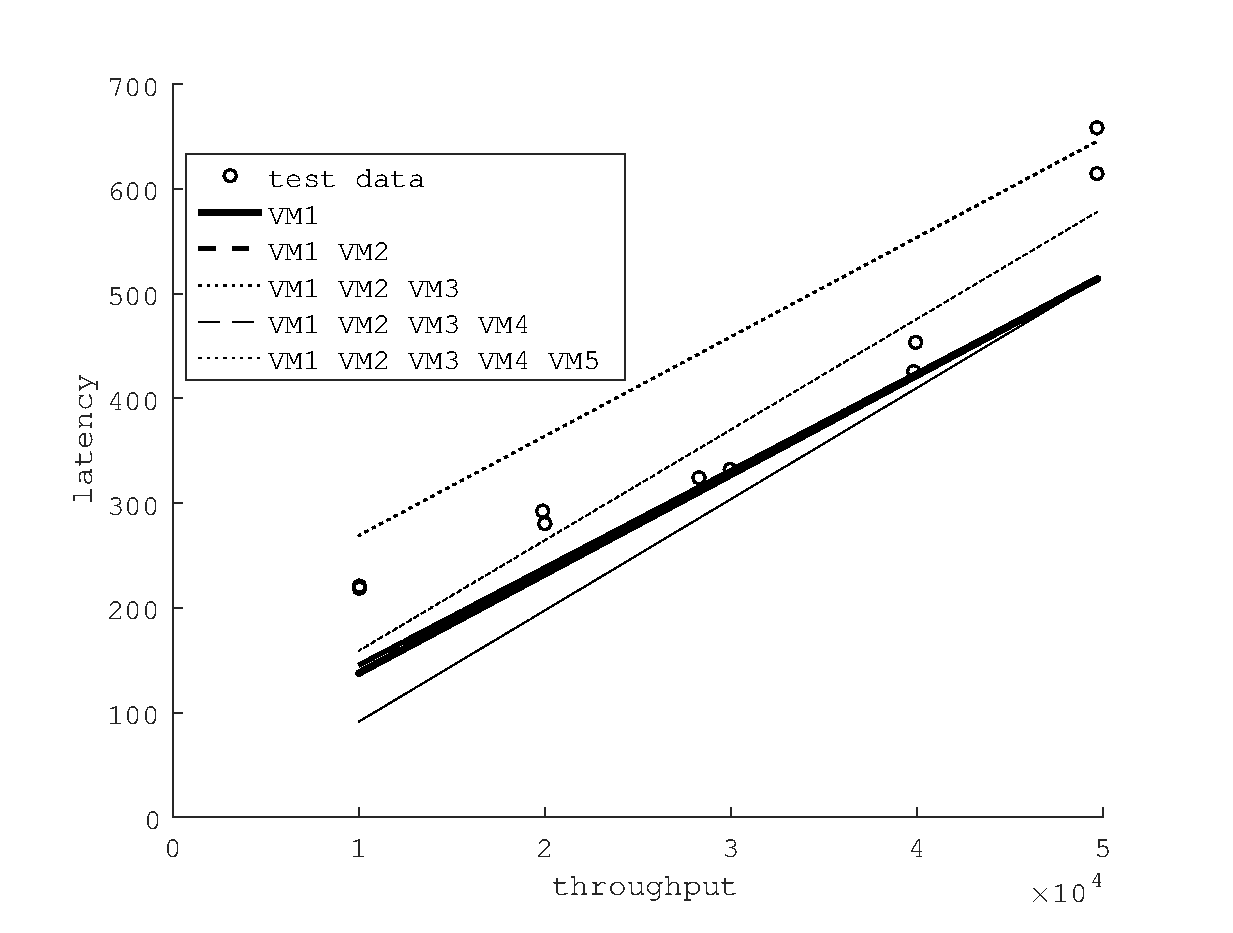
\includegraphics[scale = 0.5]{fit_read_avg_latency_r3_x_r3_2x_m3_x_r3__m3_2x_m3_.eps}
\caption{Redis average read latency vs throughput}
\label{figure:redisbarread}
\end{figure}

\begin{figure}
\centering
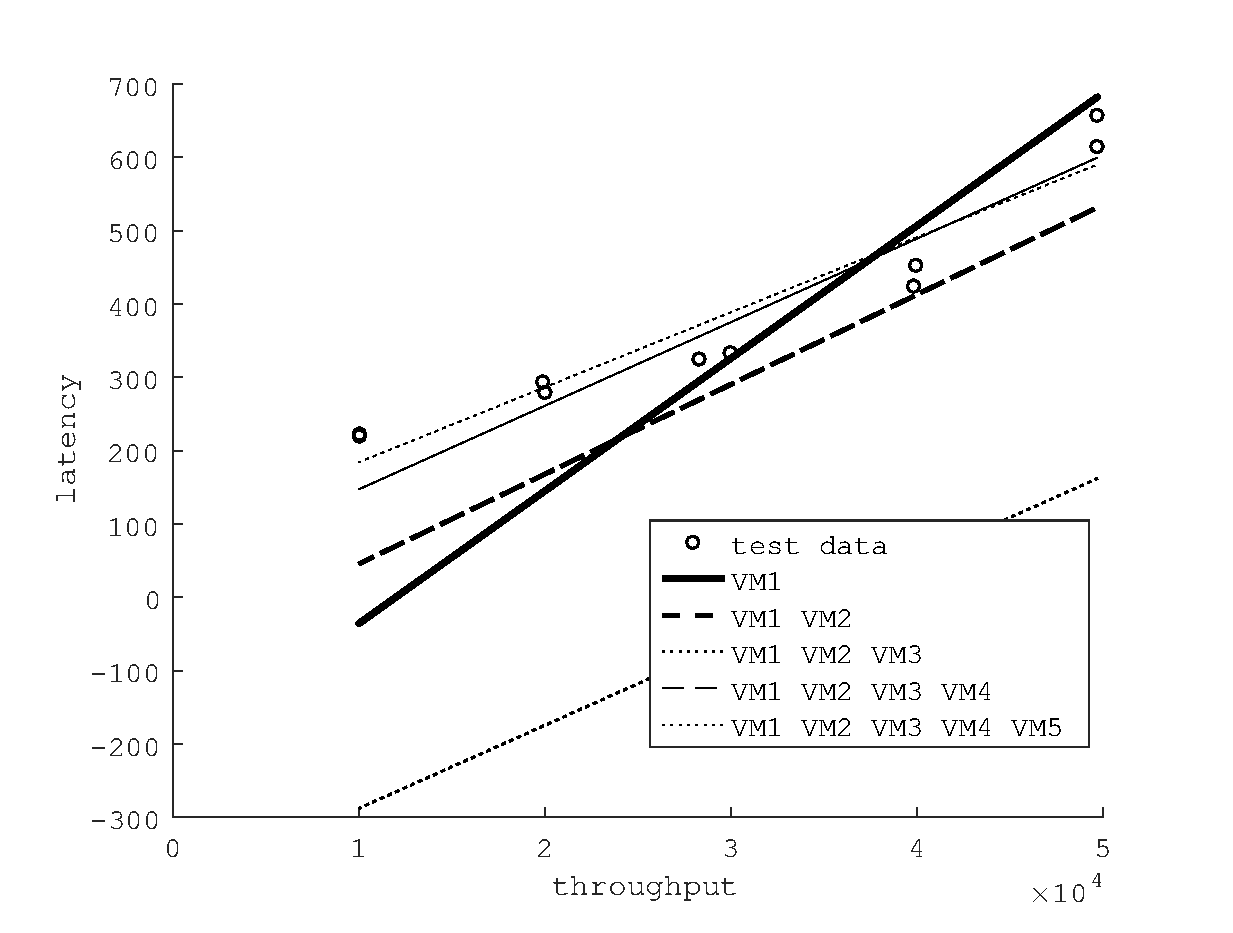
\includegraphics[scale = 0.5]{fit_read_avg_latency_r3__r3_x_m3__m3_2x_r3_2x_m3_x.eps}
\caption{Redis average read latency vs throughput}
\label{figure:redisbarread}
\end{figure}

\begin{figure}
\centering
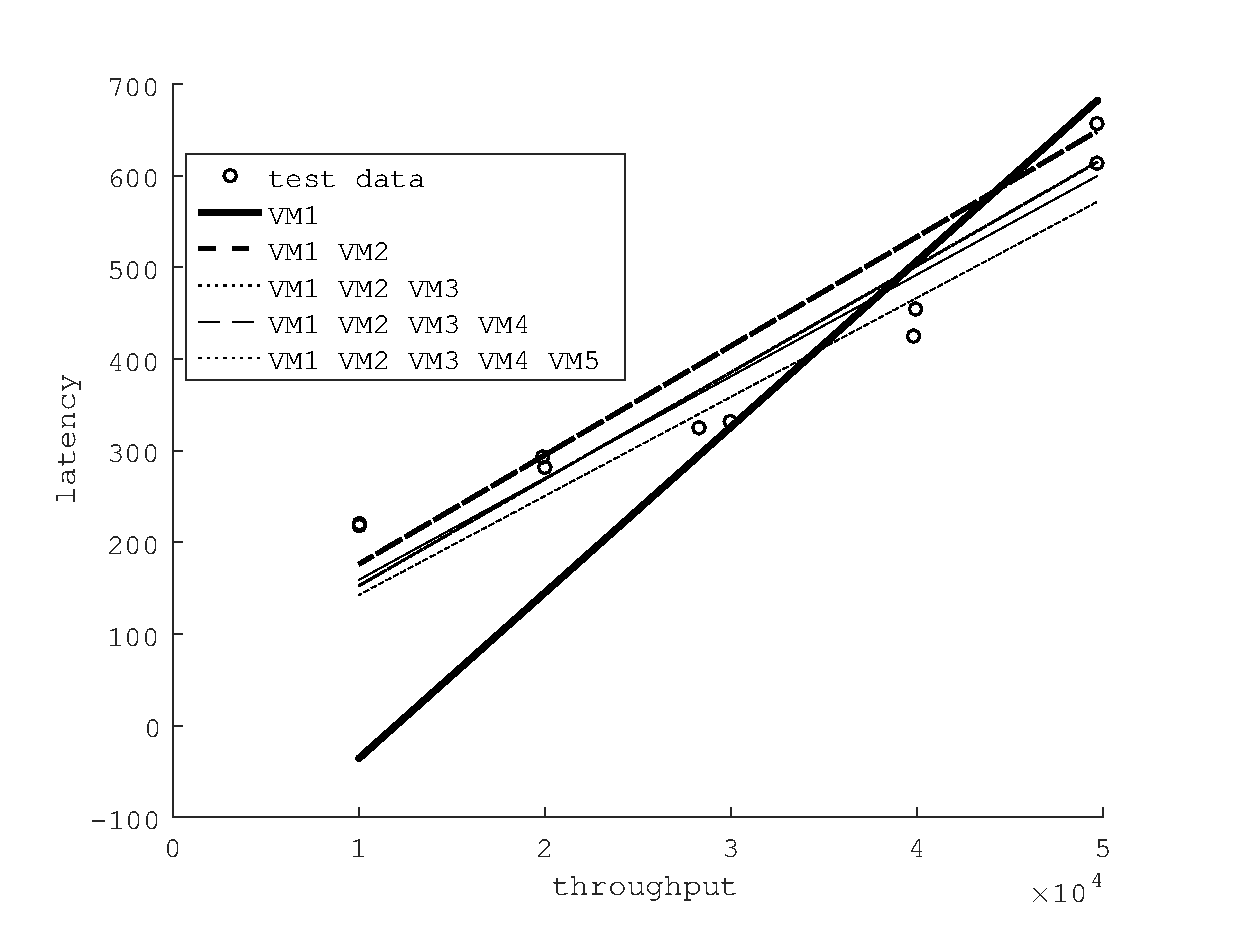
\includegraphics[scale = 0.5]{fit_read_avg_latency_r3__r3_2x_m3_2x_m3__m3_x_r3_x.eps}
\caption{Redis average read latency vs throughput}
\label{figure:redisbarread}
\end{figure}

\begin{figure}
\centering
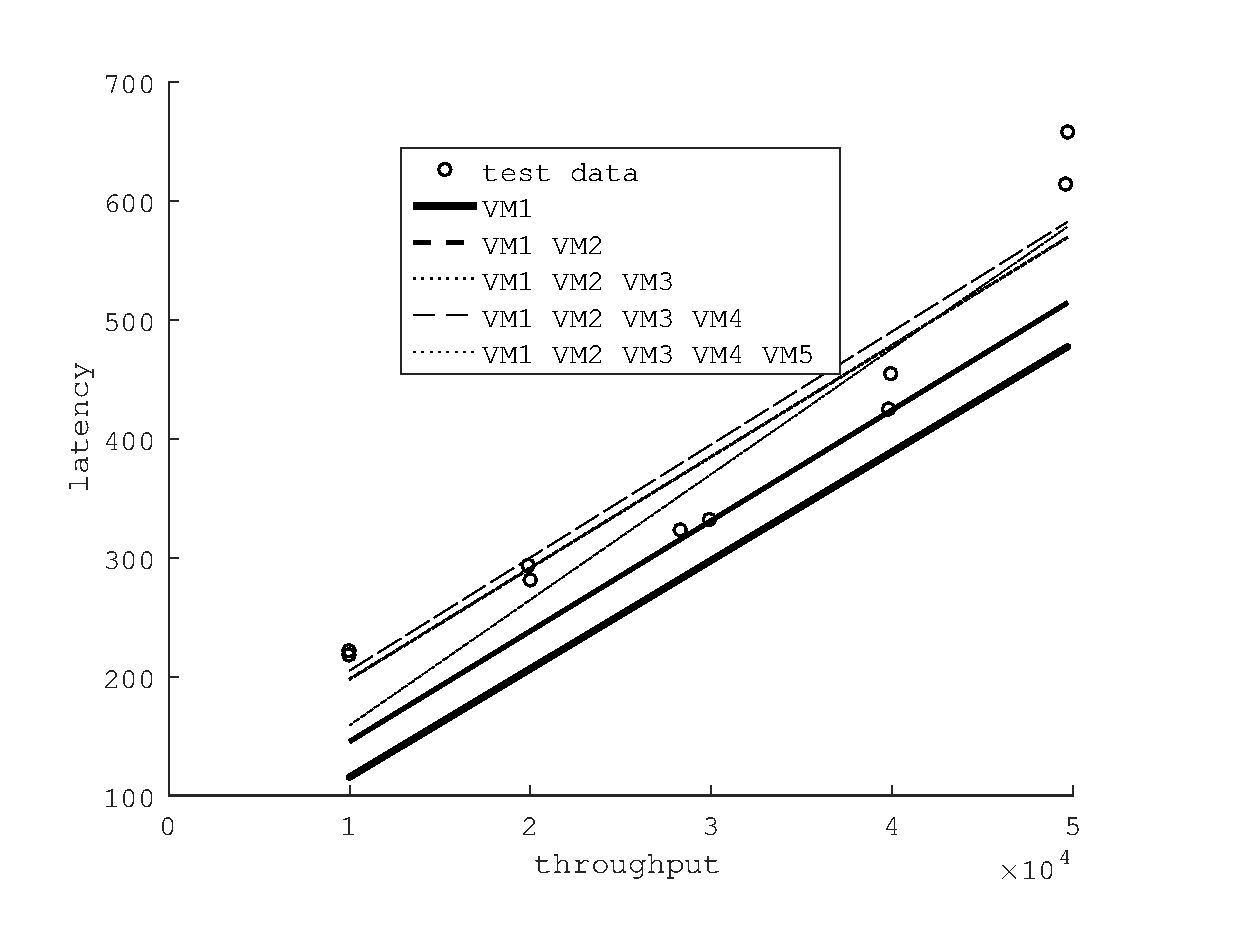
\includegraphics[scale = 0.5]{fit_read_avg_latency_r3_2x_r3_x_m3_2x_m3_x_r3__m3_.eps}
\caption{Redis average read latency vs throughput}
\label{figure:redisbarread}
\end{figure}

\begin{figure}
\centering
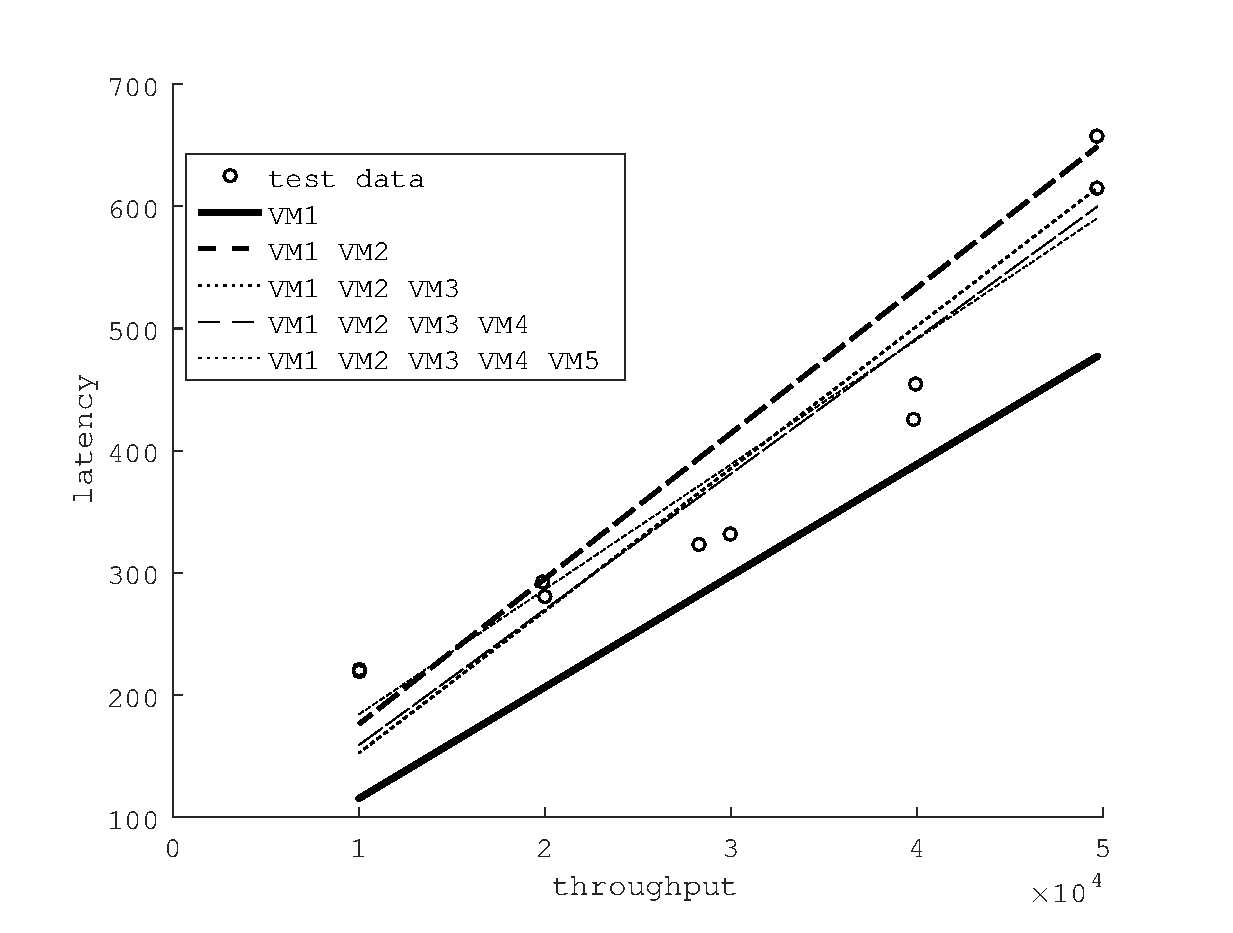
\includegraphics[scale = 0.5]{fit_read_avg_latency_r3_2x_r3__m3_2x_m3__r3_x_m3_x.eps}
\caption{Redis average read latency vs throughput}
\label{figure:redisbarread}
\end{figure}

\begin{figure}
\centering
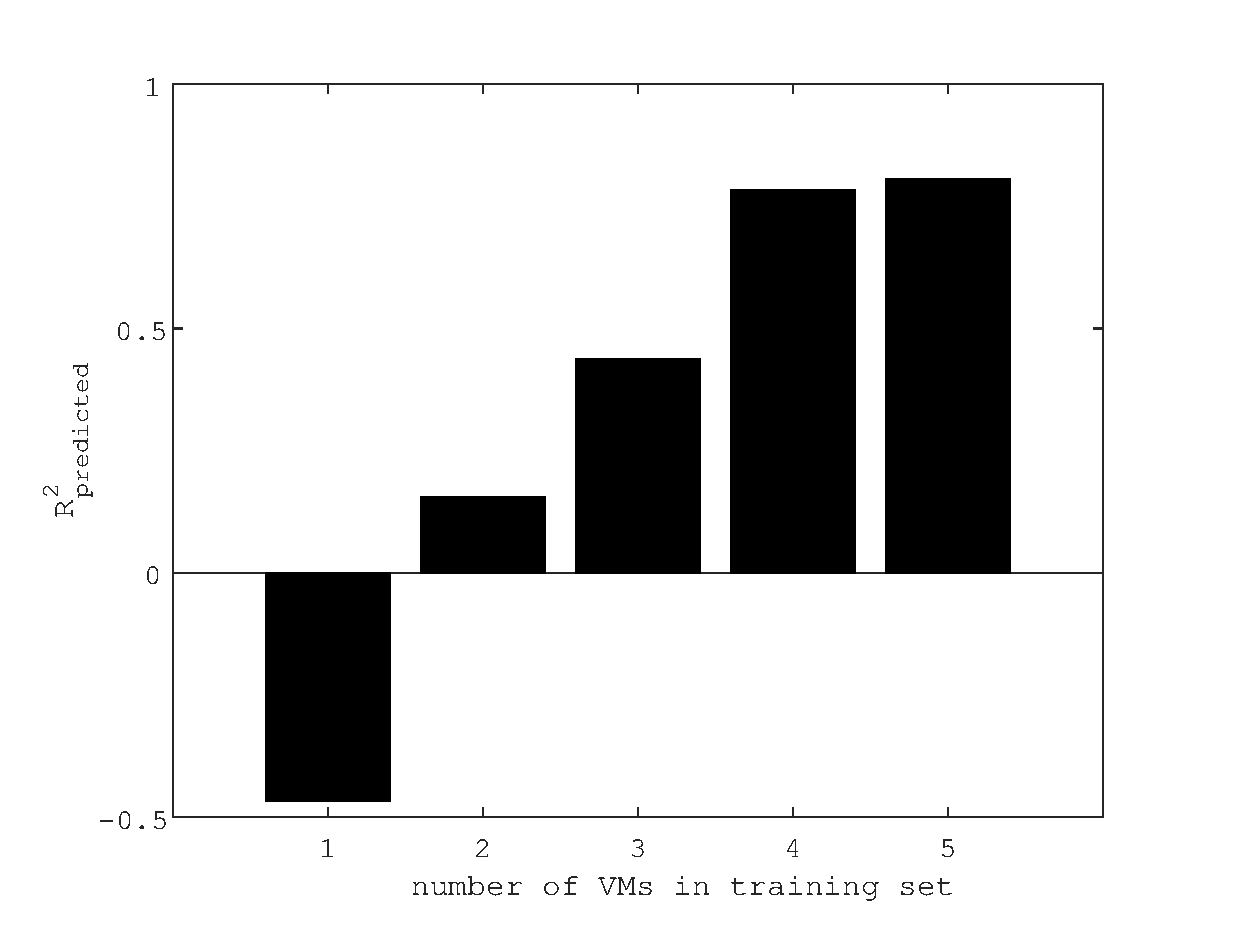
\includegraphics[scale = 0.5]{bar_read_avg_latency_r3_x_r3_2x_m3_x_r3__m3_2x_m3_.eps}
\caption{Redis R-squared vs training set}
\label{figure:redisbarread}
\end{figure}

\begin{figure}
\centering
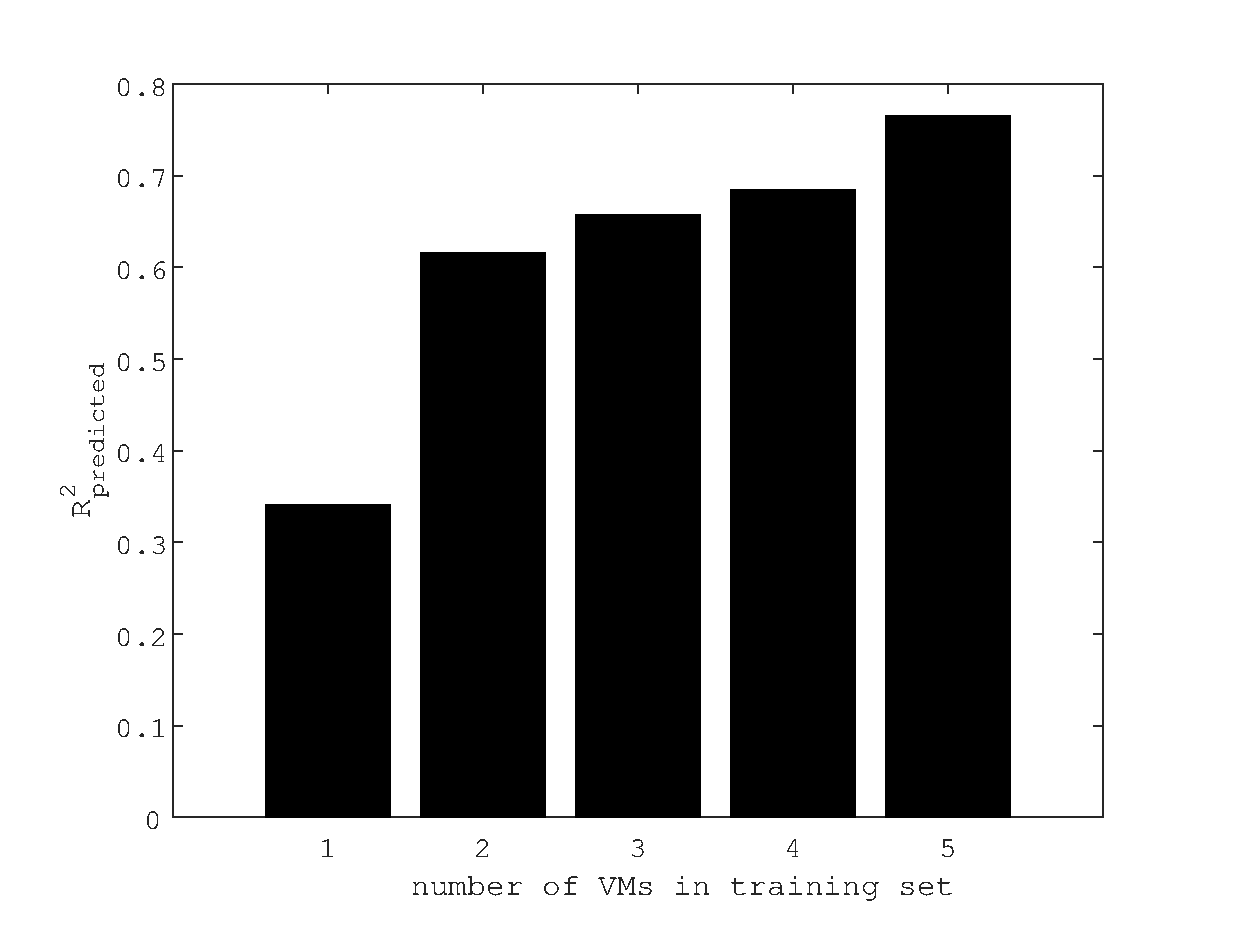
\includegraphics[scale = 0.5]{bar_read_avg_latency_r3__r3_x_m3__m3_2x_r3_2x_m3_x.eps}
\caption{Redis R-squared vs training set}
\label{figure:redisbarread}
\end{figure}

\begin{figure}
\centering
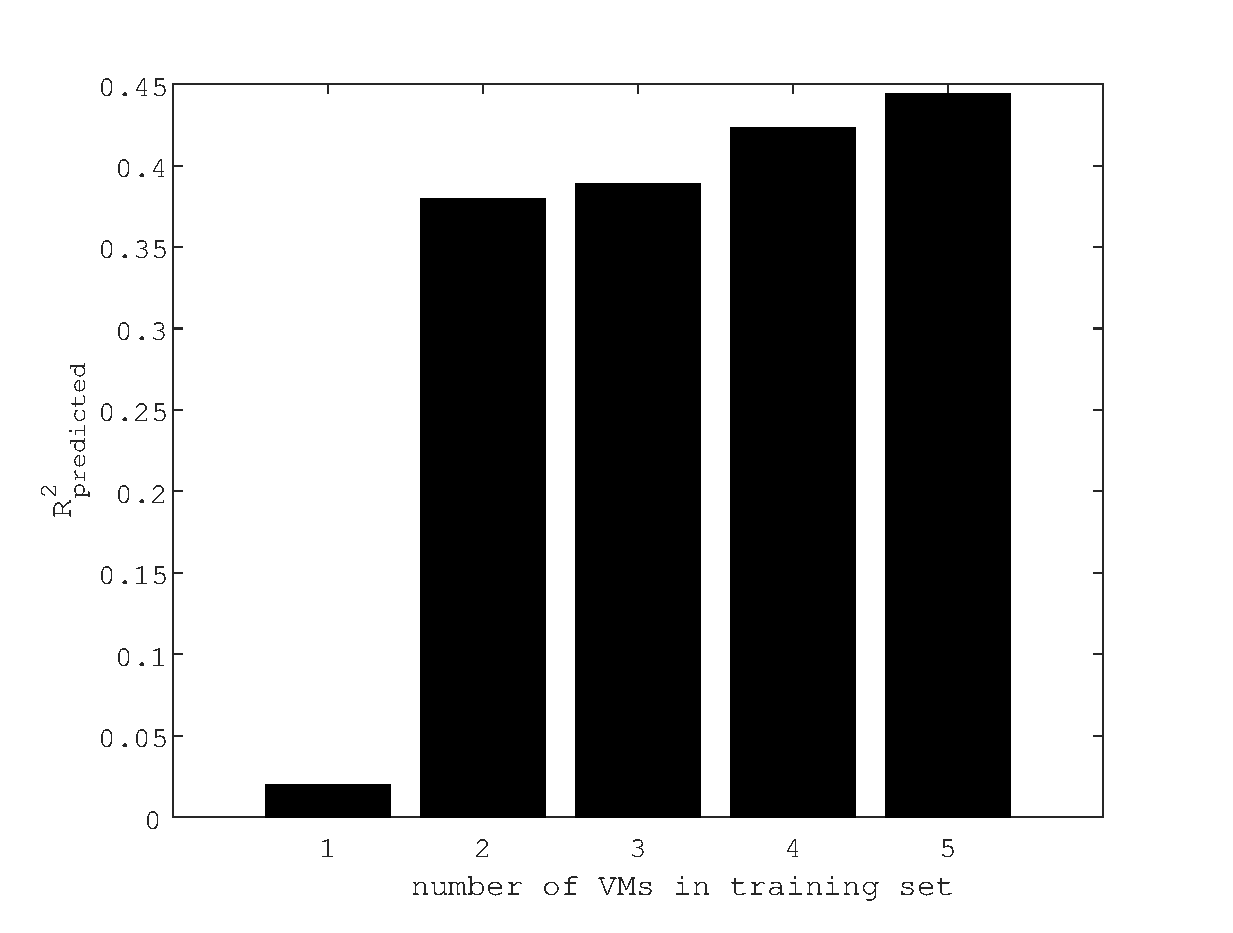
\includegraphics[scale = 0.5]{bar_read_avg_latency_r3__r3_2x_m3_2x_m3__m3_x_r3_x.eps}
\caption{Redis R-squared vs training set}
\label{figure:redisbarread}
\end{figure}

\begin{figure}
\centering
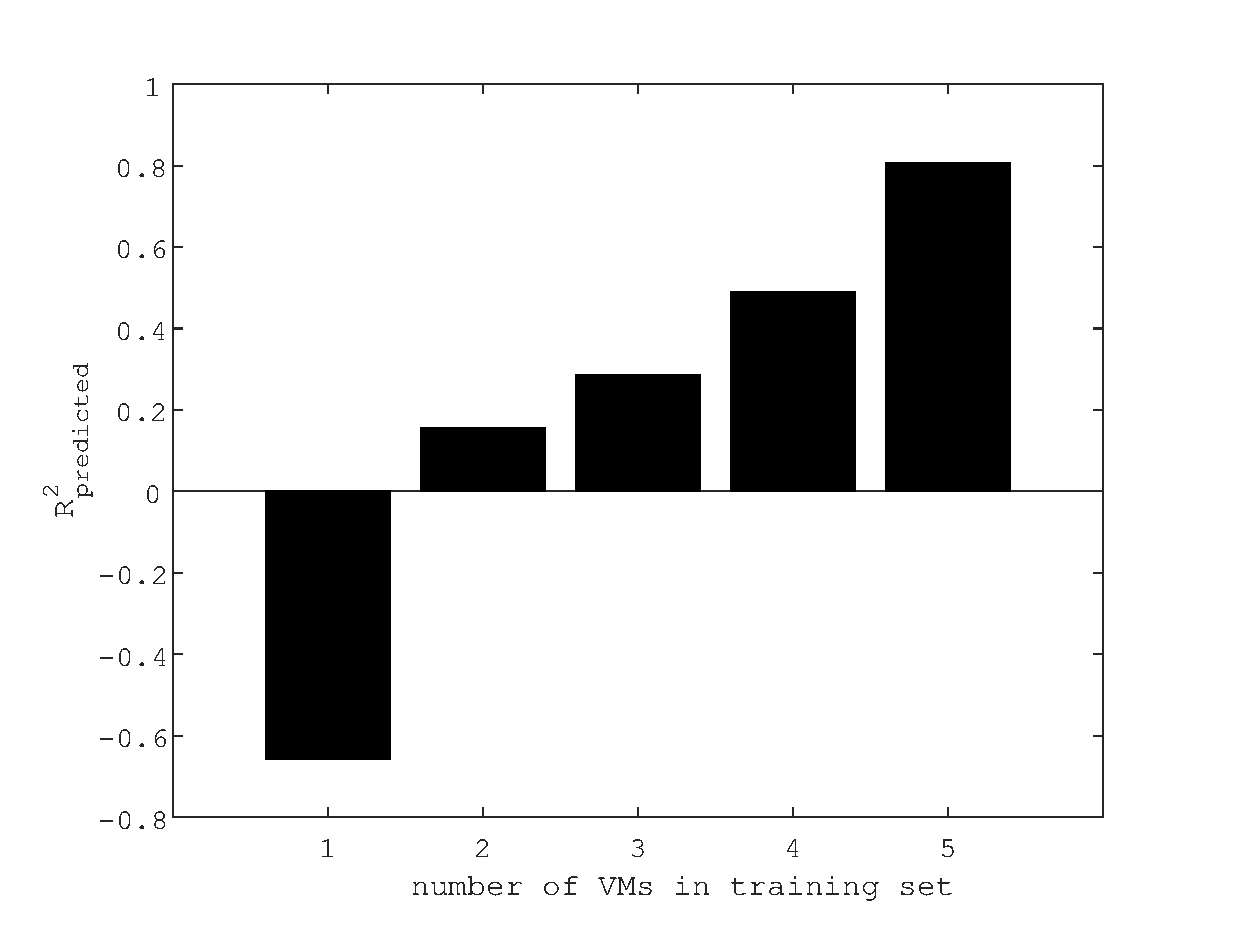
\includegraphics[scale = 0.5]{bar_read_avg_latency_r3_2x_r3_x_m3_2x_m3_x_r3__m3_.eps}
\caption{Redis R-squared vs training set}
\label{figure:redisbarread}
\end{figure}

\begin{figure}
\centering
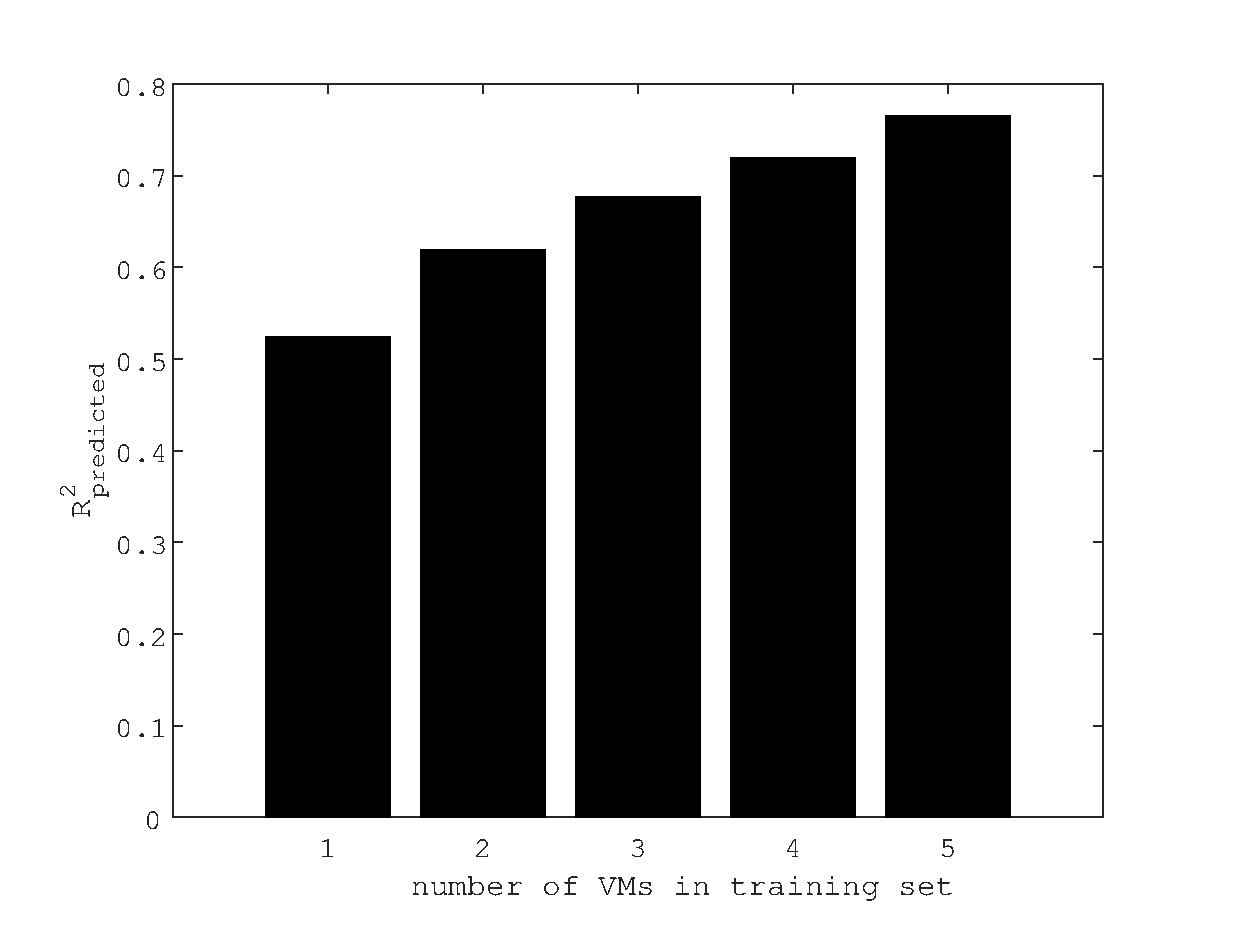
\includegraphics[scale = 0.5]{bar_read_avg_latency_r3_2x_r3__m3_2x_m3__r3_x_m3_x.eps}
\caption{Redis R-squared vs training set}
\label{figure:redisbarread}
\end{figure}

% \begin{figure}
% \centering
% 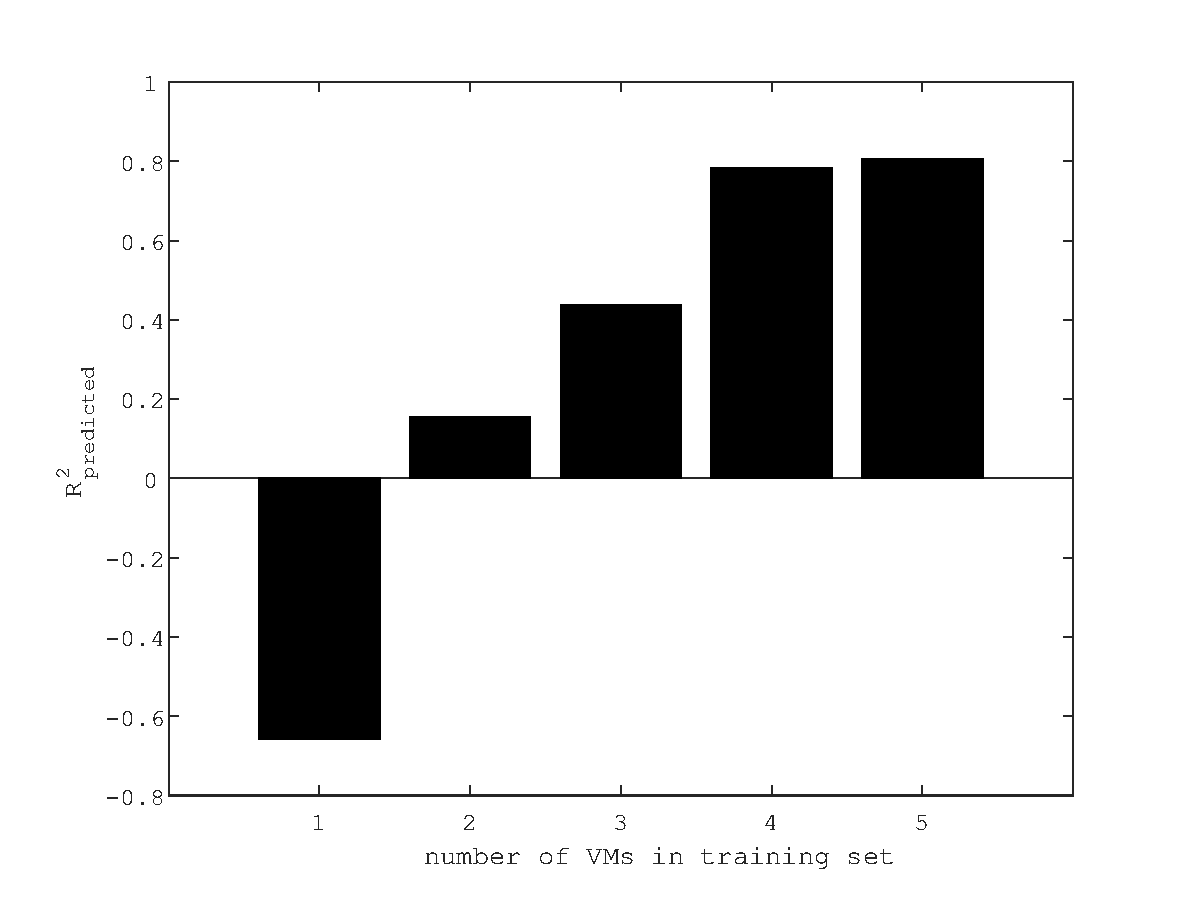
\includegraphics[scale = 0.5]{redis_read_bar.eps}
% \caption{Redis R-squared vs training set}
% \label{figure:redisbarread}
% \end{figure}

\begin{figure}
\centering
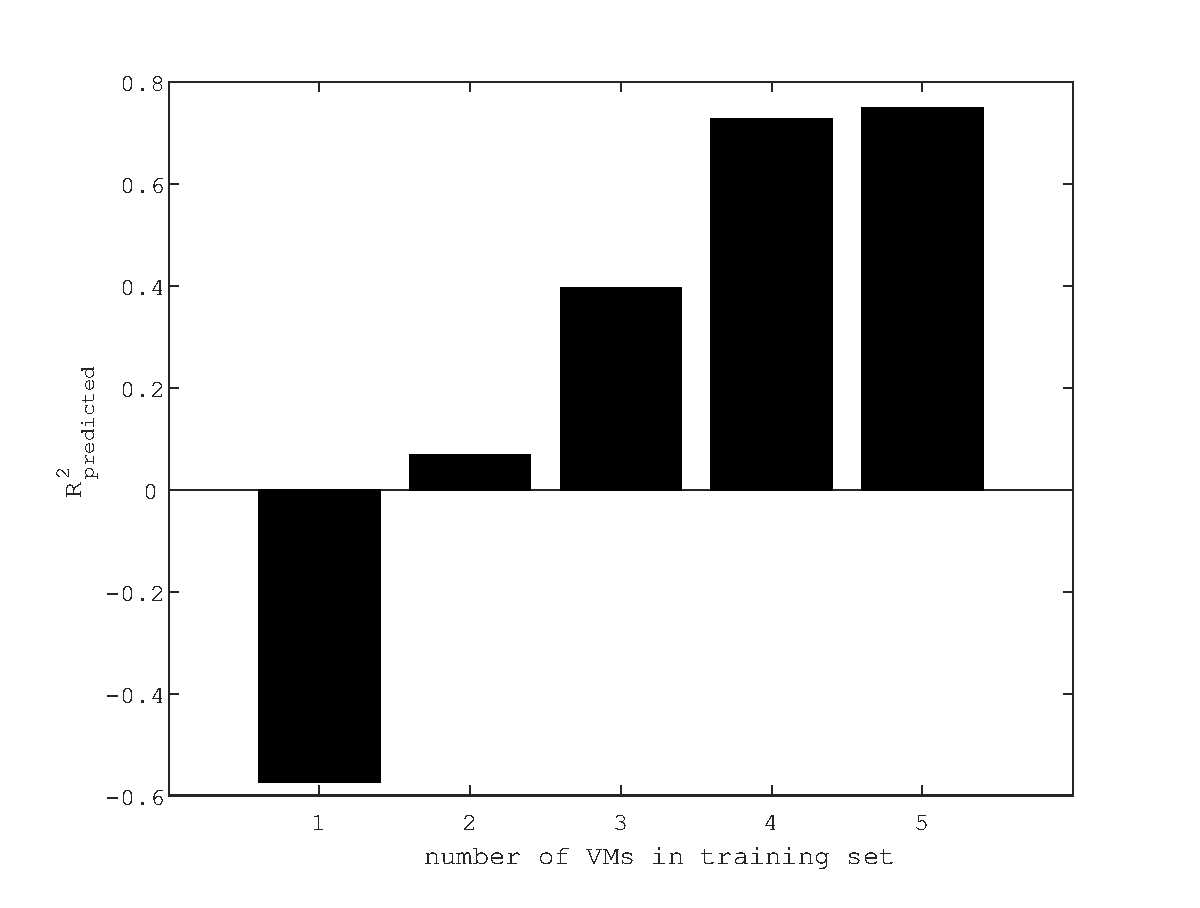
\includegraphics[scale = 0.5]{redis_write_bar.eps}
\caption{Redis R-squared vs training set}
\label{figure:redisbarwrite}
\end{figure}

% \begin{figure}
% \centering
% 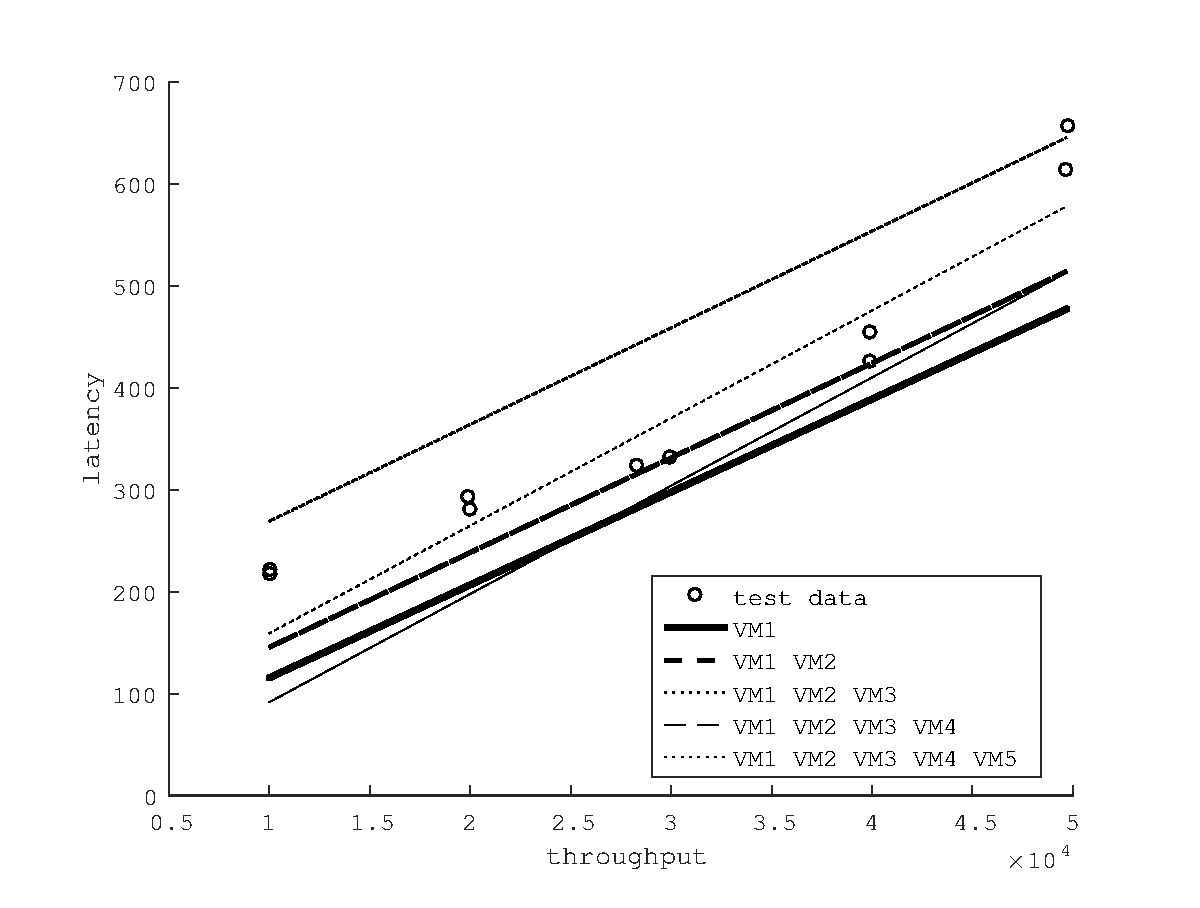
\includegraphics[scale = 0.5]{redis_read_plot.eps}
% \caption{Redis average read latency vs throughput}
% \label{figure:redisread}
% \end{figure}

% \begin{figure}
% \centering
% 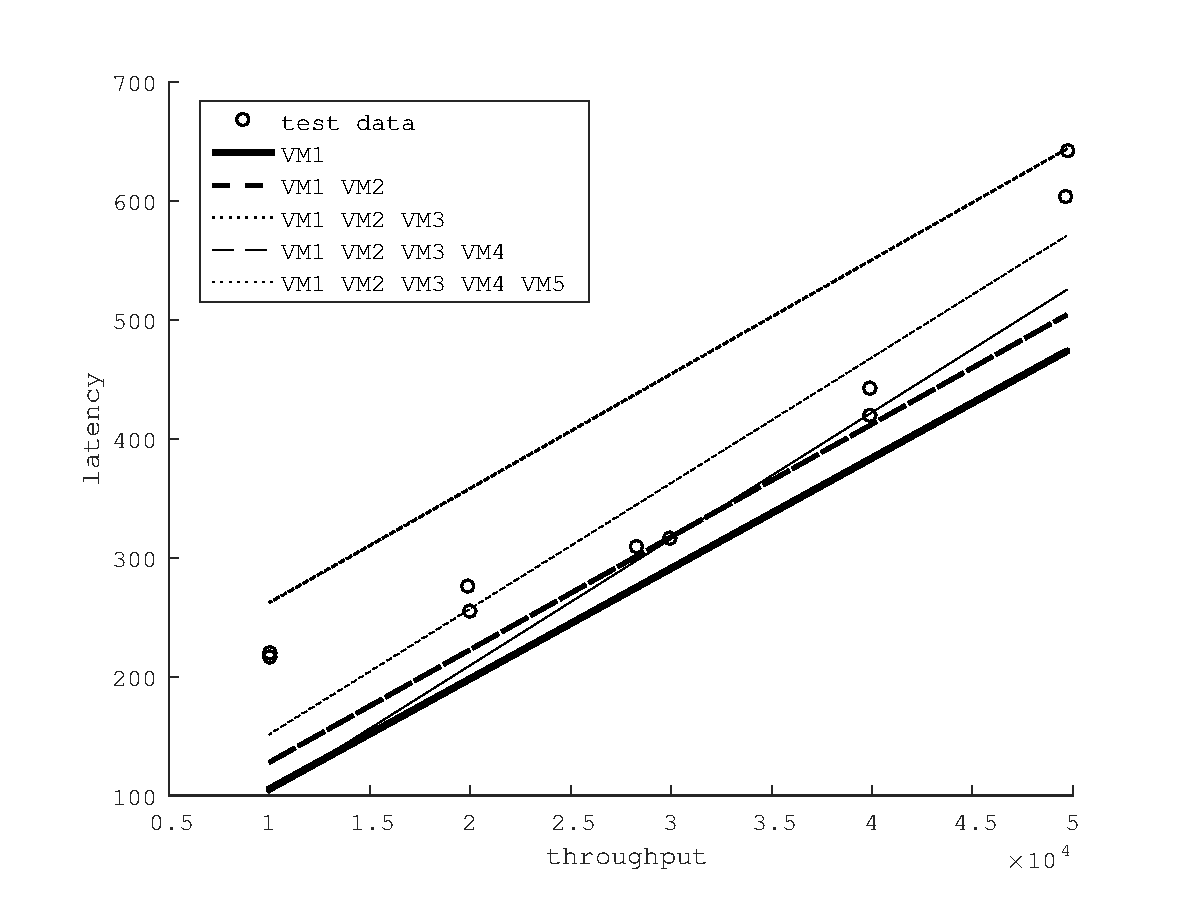
\includegraphics[scale = 0.5]{redis_write_plot.eps}
% \caption{Redis average write latency vs throughput}
% \label{figure:rediswrite}
% \end{figure}

\subsection{MySQL}

MySQL was deployed using Amazon Relational Database Service (Amazon RDS), which abstracts away the deployment and administration of OS and relationship database software.

MySQL was deployed to six VM types as listed in Table \ref{table:rdstypes}.

We tested using YCSB Workload A (50\% read, 50\% write) with a uniform distribution.

We did a multiple linear regression on the variables throughput, cores, memory, and network.  (Network performance was quantified by representing it as an dummy variable.)

We used VM type r3.2xlarge as test data, while increasing the training data in Table \ref{table:mysql}.

\begin{table}
\centering
\caption{MySQL $R_{predicted}^2$ for $VM_6$}
\begin{tabular}{|r|r|l|} \hline
$R_{read}^2$&$R_{write}^2$&Training Data\\ \hline
0 & 0& $VM_1,VM_2,VM_3$\\ \hline
0 & 0& $VM_1,VM_2,VM_3,VM_4$\\ \hline
0 & 0& $VM_1,VM_2,VM_3,V_4,V_5$\\ \hline
\hline\end{tabular}
\label{table:mysql}
\end{table}

\section{Related Work}

\begin{itemize}
   \item Chris Stewart - non-stationarity of workloads
   \item Delta modeling from CMU
   \item Graybox modeling from Wisconsin
   \item work by Shivnath Babu of Duke
\end{itemize}


\section{Lessons, Challenges, and Future Directions}

\section{Conclusions}

%\end{document}  % This is where a 'short' article might terminate


%
% The following two commands are all you need in the
% initial runs of your .tex file to
% produce the bibliography for the citations in your paper.
\bibliographystyle{abbrv}
\bibliography{sigproc}  % sigproc.bib is the name of the Bibliography in this case
% You must have a proper ".bib" file
%  and remember to run:
% latex bibtex latex latex
% to resolve all references
%
% ACM needs 'a single self-contained file'!
%

\balancecolumns
% That's all folks!
\end{document}